\documentclass[UTF-8]{article}
\usepackage{ctex}
\usepackage{geometry}
\usepackage{setspace}
\usepackage{bm}
\usepackage{siunitx}
\usepackage{amsmath}
\usepackage{amssymb}
\usepackage{hyperref}
\usepackage{graphicx}
\usepackage{listings}
\usepackage{tabularx}
\usepackage{array}
\usepackage{color}
\geometry{a4paper, bottom=2.5cm,top=2.5cm,left=2.5cm,right=2.5cm}
\title{计算物理学第一次作业报告}
\author{陈跃元}
\date{物理学院 1600011328}
%\renewcommand{\thesection}{\Roman{section}}
\renewcommand\tablename{表}
\renewcommand\figurename{图}
\newcolumntype{C}{>{\centering\arraybackslash}X}
\definecolor{backcolour}{rgb}{0.95,0.95,0.92}
\definecolor{codegreen}{rgb}{0,0.6,0}
\definecolor{codegray}{rgb}{0.5,0.5,0.5}
\definecolor{codepurple}{rgb}{0.58,0,0.82}
\lstdefinestyle{mystyle}{
	commentstyle=\color{codegreen},
	keywordstyle=\color{magenta},
	numberstyle=\tiny\color{codegray},
	stringstyle=\color{codepurple},
	basicstyle=\ttfamily\footnotesize,
	breakatwhitespace=false,         
	breaklines=true,                 
	captionpos=b,                    
	keepspaces=true,                 
	numbers=left,                    
	numbersep=5pt,                  
	showspaces=false,                
	showstringspaces=false,
	showtabs=false,                  
	tabsize=4
}
\lstset{style=mystyle}
\hypersetup{colorlinks=true}
\begin{document}
	\maketitle
\section{双精度浮点数和其IEEE754编码的互相转化}
\subsection{问题描述}
实现任意十进制数于其规范化的二进制双精度浮点数编码间的相互转换.具体而言,输入一个双精度浮点数,需要给出它按照IEEE754标准的编码;输入一个64位,由‘0’和‘1’组成的字符串,将它按照IEEE754标准转化为双精度浮点数.
\subsection{算法}
\subsubsection{双精度浮点数转编码}
有两种可行的算法:
\begin{enumerate}
\item 按定义转换
	\begin{itemize}
		\item 确定符号位(若$x==0$直接返回全零),exponent初始值设为1023.
		\item (确定exponent)判断$x\geqslant1$?
		\begin{itemize}
			\item Yes \\
			不断重复$x/=2,\quad\text{exponent}++$,直到$x<2$.
			\item No \\
			不断重复$x*=2,\quad\text{exponent}--$,直到$x>=1$.
		\end{itemize}
		\item $x--$
		\item (小数的二进制转换)从$i=12$开始,不断重复$x*=2,\quad s[i]=x\%1,\quad i++$,直至将$s$的小数部分52位全部填满.
		\item 返回$s$.
	\end{itemize}
	这一算法比起将$x$分解为整数部分和小数部分分别转换的效率要更高(同为$O(\lg n)$级别, 但常数比分开转换要小), 且在大数情形下, 不会出现分解出的整数部分过大造成的overflow. 
\item 利用强制指针类型转换\\
	这一算法某种程度上是一种投机取巧的办法. 在\texttt{C++}中, \texttt{double }类型和\texttt{long long }类型都是由8个字节来存储的, 且\texttt{double }类型在内存中的存储方式就是按照IEEE 754标准执行的, 故可以通过将指向$x$的\texttt{double }类指针强制转化为\texttt{long long }类指针, 随后将这一\texttt{long long }按照整数的二进制转换来得到编码.
\end{enumerate}
\subsubsection{编码转双精度浮点数}
这时的算法相当于将上面两个算法倒过来.
\begin{enumerate}
\item 按定义转换
\begin{itemize}
	\item (确定小数)将$s$的后52位按照二进制小数的规则转化为$x$.
	\item $x++$
	\item (确定exponent)将exponent部分计算出来.判断: 
	\begin{itemize}
		\item $\text{exponent}==0$ \\
		返回$x=0$.
		\item $\text{exponent}>=1023$ \\
		不断重复$x*=2,\quad\text{exponent}--$,直到$\text{exponent}=1023$.
		\item $0<\text{exponent}<1023$ \\
		不断重复$x/=2,\quad\text{exponent}++$,直到$\text{exponent}=1023$.
	\end{itemize}
	\item 若符号位为1, $x*=-1$.
	\item 返回$x$.
\end{itemize}

\item 利用强制指针类型转换\\
将$s$按照整数的二进制转化规则转化为\texttt{long long }类型的$x$, 并将指向$x$的\texttt{long long }指针强制类型转换为\texttt{double }指针,返回指针所指的双精度浮点数.
\end{enumerate}
源代码见附录\ref{subsec:Q_1},或\texttt{src/Problem\_1/main.cpp}.
\subsection{结果}
\begin{figure}[h]
	\centering
	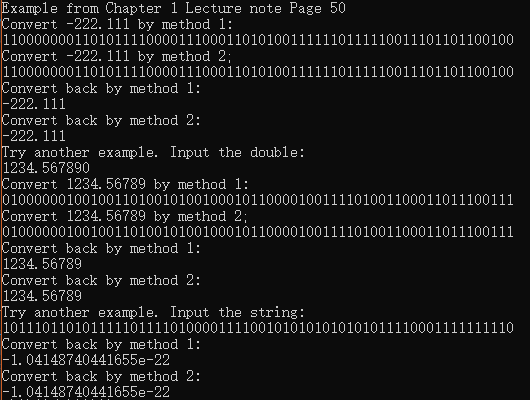
\includegraphics[width=0.7\textwidth]{Q_1.png}
	\caption{第一题的结果}
	\label{fig:Q_1}
\end{figure}
运行如图\ref{fig:Q_1}所示.两种方法得到的结果相同.

\section{带权的高斯积分}
\subsection{问题描述}
构造下列三个高斯积分的节点和权重.
\begin{equation}
	\int_{0}^{1} \sqrt{x} f(x) d x \approx A_{0} f\left(x_{0}\right)+A_{1} f\left(x_{1}\right)
	\label{eq:1}
\end{equation}
\begin{equation}
\int_{0}^{1} \sqrt{x} f(x) d x \approx A_{0} f\left(x_{0}\right)+A_{1} f\left(x_{1}\right)+A_{2} f\left(x_{2}\right)
\label{eq:2}
\end{equation}
\begin{equation}
\int_{-1}^{1}\left(1+x^{2}\right) f(x) d x \approx A_{0} f\left(x_{0}\right)+A_{1} f\left(x_{1}\right)
\label{eq:3}
\end{equation}
\subsection{推导和结果}
对(\ref{eq:1}),对于节点$x_i$, 应满足对所有$0\leqslant k\leqslant n$,
\begin{equation}
\label{eq:4}
	\int_{0}^{1}\sqrt{x}\left[ \prod_{i=0}^n(x-x_i)\right] P_{k}(x) d x=0
\end{equation}
即
\begin{equation}
	\left\lbrace
	\begin{split}
	\frac{1}{7}-\frac{x_0}{5}-\frac{x_1}{5}+\frac{x_0 x_1}{3}&=0\\
	\frac{1}{9}-\frac{x_0}{7}-\frac{x_1}{7}+\frac{x_0 x_1}{5}&=0
	\end{split}
	\right.
\end{equation}
解得$x_0=\frac{1}{63}(35-2 \sqrt{70})\approx 0.289949,  x_1=\frac{1}{63}(35+2 \sqrt{70})\approx 0.821162$. 带入原式, 为使所有阶数$\leqslant1$的多项式积分为准确值, 应有
\begin{equation}
	\left\lbrace
	\begin{split}
	A_0+A_1&=\frac{2}{3}\\
	A_0 x_0+A_1 x_1&=\frac{2}{5}
	\end{split}
	\right.
\end{equation}
解得$A_0\approx0.277556, A_1\approx0.389111$.

对(\ref{eq:2}),同样有(\ref{eq:4})的要求,即
\begin{equation}
\left\lbrace
\begin{split}
-\frac{2}{3} a b c+\frac{2}{5}(ab+bc+ac)-\frac{2}{7}(a+b+c)+\frac{2}{9}&=0\\
-\frac{2}{5} a b c+\frac{2}{7}(ab+bc+ac)-\frac{2}{9}(a+b+c)+\frac{2}{11}&=0\\
-\frac{2}{21}abc+\frac{2}{15}(ab+bc+ca)-\frac{10}{77}(a+b+c)+\frac{14}{117}&=0
\end{split}
\right.
\end{equation}
解得$x_0=\frac{1}{63}(35-2 \sqrt{70})\approx 0.289949,  x_1=\frac{1}{63}(35+2 \sqrt{70})\approx 0.821162$. 带入原式, 为使所有阶数$\leqslant1$的多项式积分为准确值, 应有
\begin{equation}
\left\lbrace
\begin{split}
A_0+A_1&=\frac{2}{3}\\
A_0 x_0+A_1 x_1&=\frac{2}{5}
\end{split}
\right.
\end{equation}
解得$A_0\approx0.277556, A_1\approx0.389111$.

\section{衰变}
\subsection{问题描述}
两类核A和B发生衰变, 初始时刻$N_A=N_B=1$, 满足
\begin{equation} 
\frac{d N_{A}}{d t}=-\frac{N_{A}}{\tau_{A}}
\end{equation}
\begin{equation}
	\frac{d N_{B}}{d t}=\frac{N_{A}}{\tau_{A}}-\frac{N_{B}}{\tau_{B}}
\end{equation}
编写程序求解耦合微分方程组, 并和解析解比较.
\subsection{算法}
解析解: 
\begin{equation}
	N_A=\exp(-\frac{t}{\tau_{A}}),\quad N_B=\frac{\tau_{A}\exp(-\frac{t}{\tau_{B}})+\tau_{B}(\exp(-\frac{t}{\tau_{A}})-2\exp(-\frac{t}{\tau_{B}}))}{\tau_{A}-\tau_{B}}
\end{equation}
笔者考虑了下面四种不同的算法(伪代码中将$N_A$和$N_B$分别记作\texttt{a}, \texttt{b}): 
\begin{enumerate}
\item Naive iteration
\begin{lstlisting}
	a[n] = a[n-1] - delta * a[n-1] / tau_a
	b[n] = b[n-1] + delta * (a[n-1] / tau_a - b[n-1] / tau_b)
\end{lstlisting}
其中\texttt{n }是迭代步数, \texttt{delta }是时间的步长, \texttt{tau\_a }和\texttt{tau\_b }的意义不言自明,下同.
\item Naive iteration, 但对$N_B$迭代时, $N_A$取前后两次的$N_A$的平均值.
\begin{lstlisting}
	a[n] = a[n-1] - delta * a[n-1] / tau_a
	b[n] = b[n-1] + delta * ((a[n] + a[n-1]) / (2 * tau_a) - b[n-1] / tau_b)
\end{lstlisting}
\item 对$N_A$用RK-4, 对$N_B$用Naive iteration, 但$N_A$的值取两次迭代的平均值.
\begin{lstlisting}
	k[0] = - delta * a[n-1] / tau_a
	k[1] = - delta * (a[n-1] + k[0] / 2) / tau_a
	k[2] = - delta * (a[n-1] + k[1] / 2) / tau_a
	k[3] = - delta * (a[n-1] + k[2]) / tau_a
	a[n] = a[n-1] + (k[0] + 2 * k[1] + 2 * k[2] + k[3]) / 6
	b[n] = b[n-1] + delta * ((a[n-1] + a[n]) / (2 * tau_a) - b[n-1] / tau_b)
\end{lstlisting}
\item 对$N_A$用RK-4, 然后再对$N_B$用RK-4.
\begin{lstlisting}
	k[0] = -delta * a[n-1] / tau_a
	k[1] = -delta * (a[n-1] + k[0] / 2) / tau_a
	k[2] = -delta * (a[n-1] + k[1] / 2) / tau_a
	k[3] = -delta * (a[n-1] + k[2]) / tau_a
	a[n] = a[n-1] + (k[0] + 2 * k[1] + 2 * k[2] + k[3]) / 6

	k[0] = delta * (a[n-1] / tau_a - b[n-1] / tau_b);
	k[1] = delta * ((a[n-1] + a[n]) / (2 * tau_a) - (b[n-1] + k[0] / 2) / tau_b)
	// Explicit time dependent in N_A, linear intrapolate
	k[2] = delta * ((a[n-1] + a[n]) / (2 * tau_a) - (b[n-1] + k[1] / 2) / tau_b)
	// Explicit time dependent in N_A, linear intrapolate
	k[3] = delta * (a[n] / tau_a - (b[n-1] + k[2]) / tau_b)
	b[n] = b[n-1] + (k[0] + 2 * k[1] + 2 * k[2] + k[3]) / 6
\end{lstlisting}
需要注意一点, 在得到\texttt{a[n]}以后, 代入计算$N_B$时, RK-4要求\texttt{k[1] }和\texttt{k[2] }中取\\ \texttt{t[n] + delta / 2 }时的$N_A$,但这一时刻并不在迭代的时刻中, 考虑到\texttt{delta}较小, 期间$N_A$的变化可以近似看做线性的, 故通过线性插值得到\texttt{t[n] + delta / 2 }时的$N_A$.
\end{enumerate}
源代码见附录\ref{subsec:Q_3},或\texttt{src/Problem\_3/main.cpp}.
\subsection{结果}
\subsubsection{几种方法的比较}
笔者首先比较了不同算法在$\tau_{A}=\SI{1}{\second}, \tau_{B}=\SI{10}{\second}, \Delta t=\SI{0.2}{\second}$的情况下的误差, 以找到其中误差最小的方法.图\ref{fig:Q-3-1}、\ref{fig:Q-3-2}、\ref{fig:Q-3-3}分别给出了各个方法的计算结果、相对误差和绝对误差. 表\ref{table:1}中列出了各种方法的最大相对误差. 很显然, 第四种算法的误差相比于剩下三种方法的误差要小得多, 故之后的分析都基于第四种方法.
\begin{figure}[h]
	\centering
	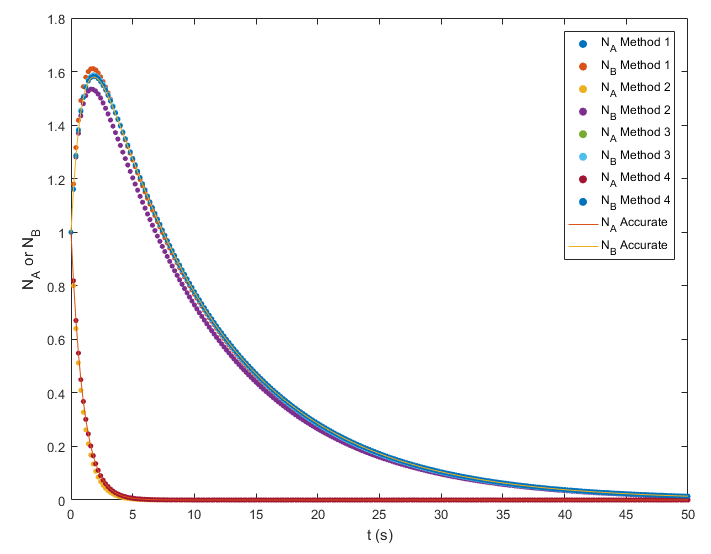
\includegraphics[width=0.6\textwidth]{Q_3_1.png}
	\caption{不同方法在$\tau_{A}=\SI{1}{\second}, \tau_{B}=\SI{10}{\second}, \Delta t=\SI{0.2}{\second}$的情况下的结果}
	\label{fig:Q-3-1}
\end{figure}
\begin{table}[h]
	\caption{不同方法在$\tau_{A}=\SI{1}{\second}, \tau_{B}=\SI{10}{\second}, \Delta t=\SI{0.2}{\second}$的情况下的最大相对误差(绝对值)}
	\vspace{1ex}
	\centering
	\begin{spacing}{1.5}
		\begin{tabularx}{\textwidth}{CCCCC}
			\hline\hline
			& Method 1 & Method 2 & Method 3 & Method 4\\
			\hline
			$N_A$ & 99.69\% & 99.69\% & 0.10\% & 0.10\% \\
			$N_B$ & 4.95\% & 9.94\% & 4.18\% & 0.22\%\\ 
			\hline\hline
		\end{tabularx}
	\end{spacing}
	\label{table:1}
\end{table}
\begin{figure}[h]
	\centering
	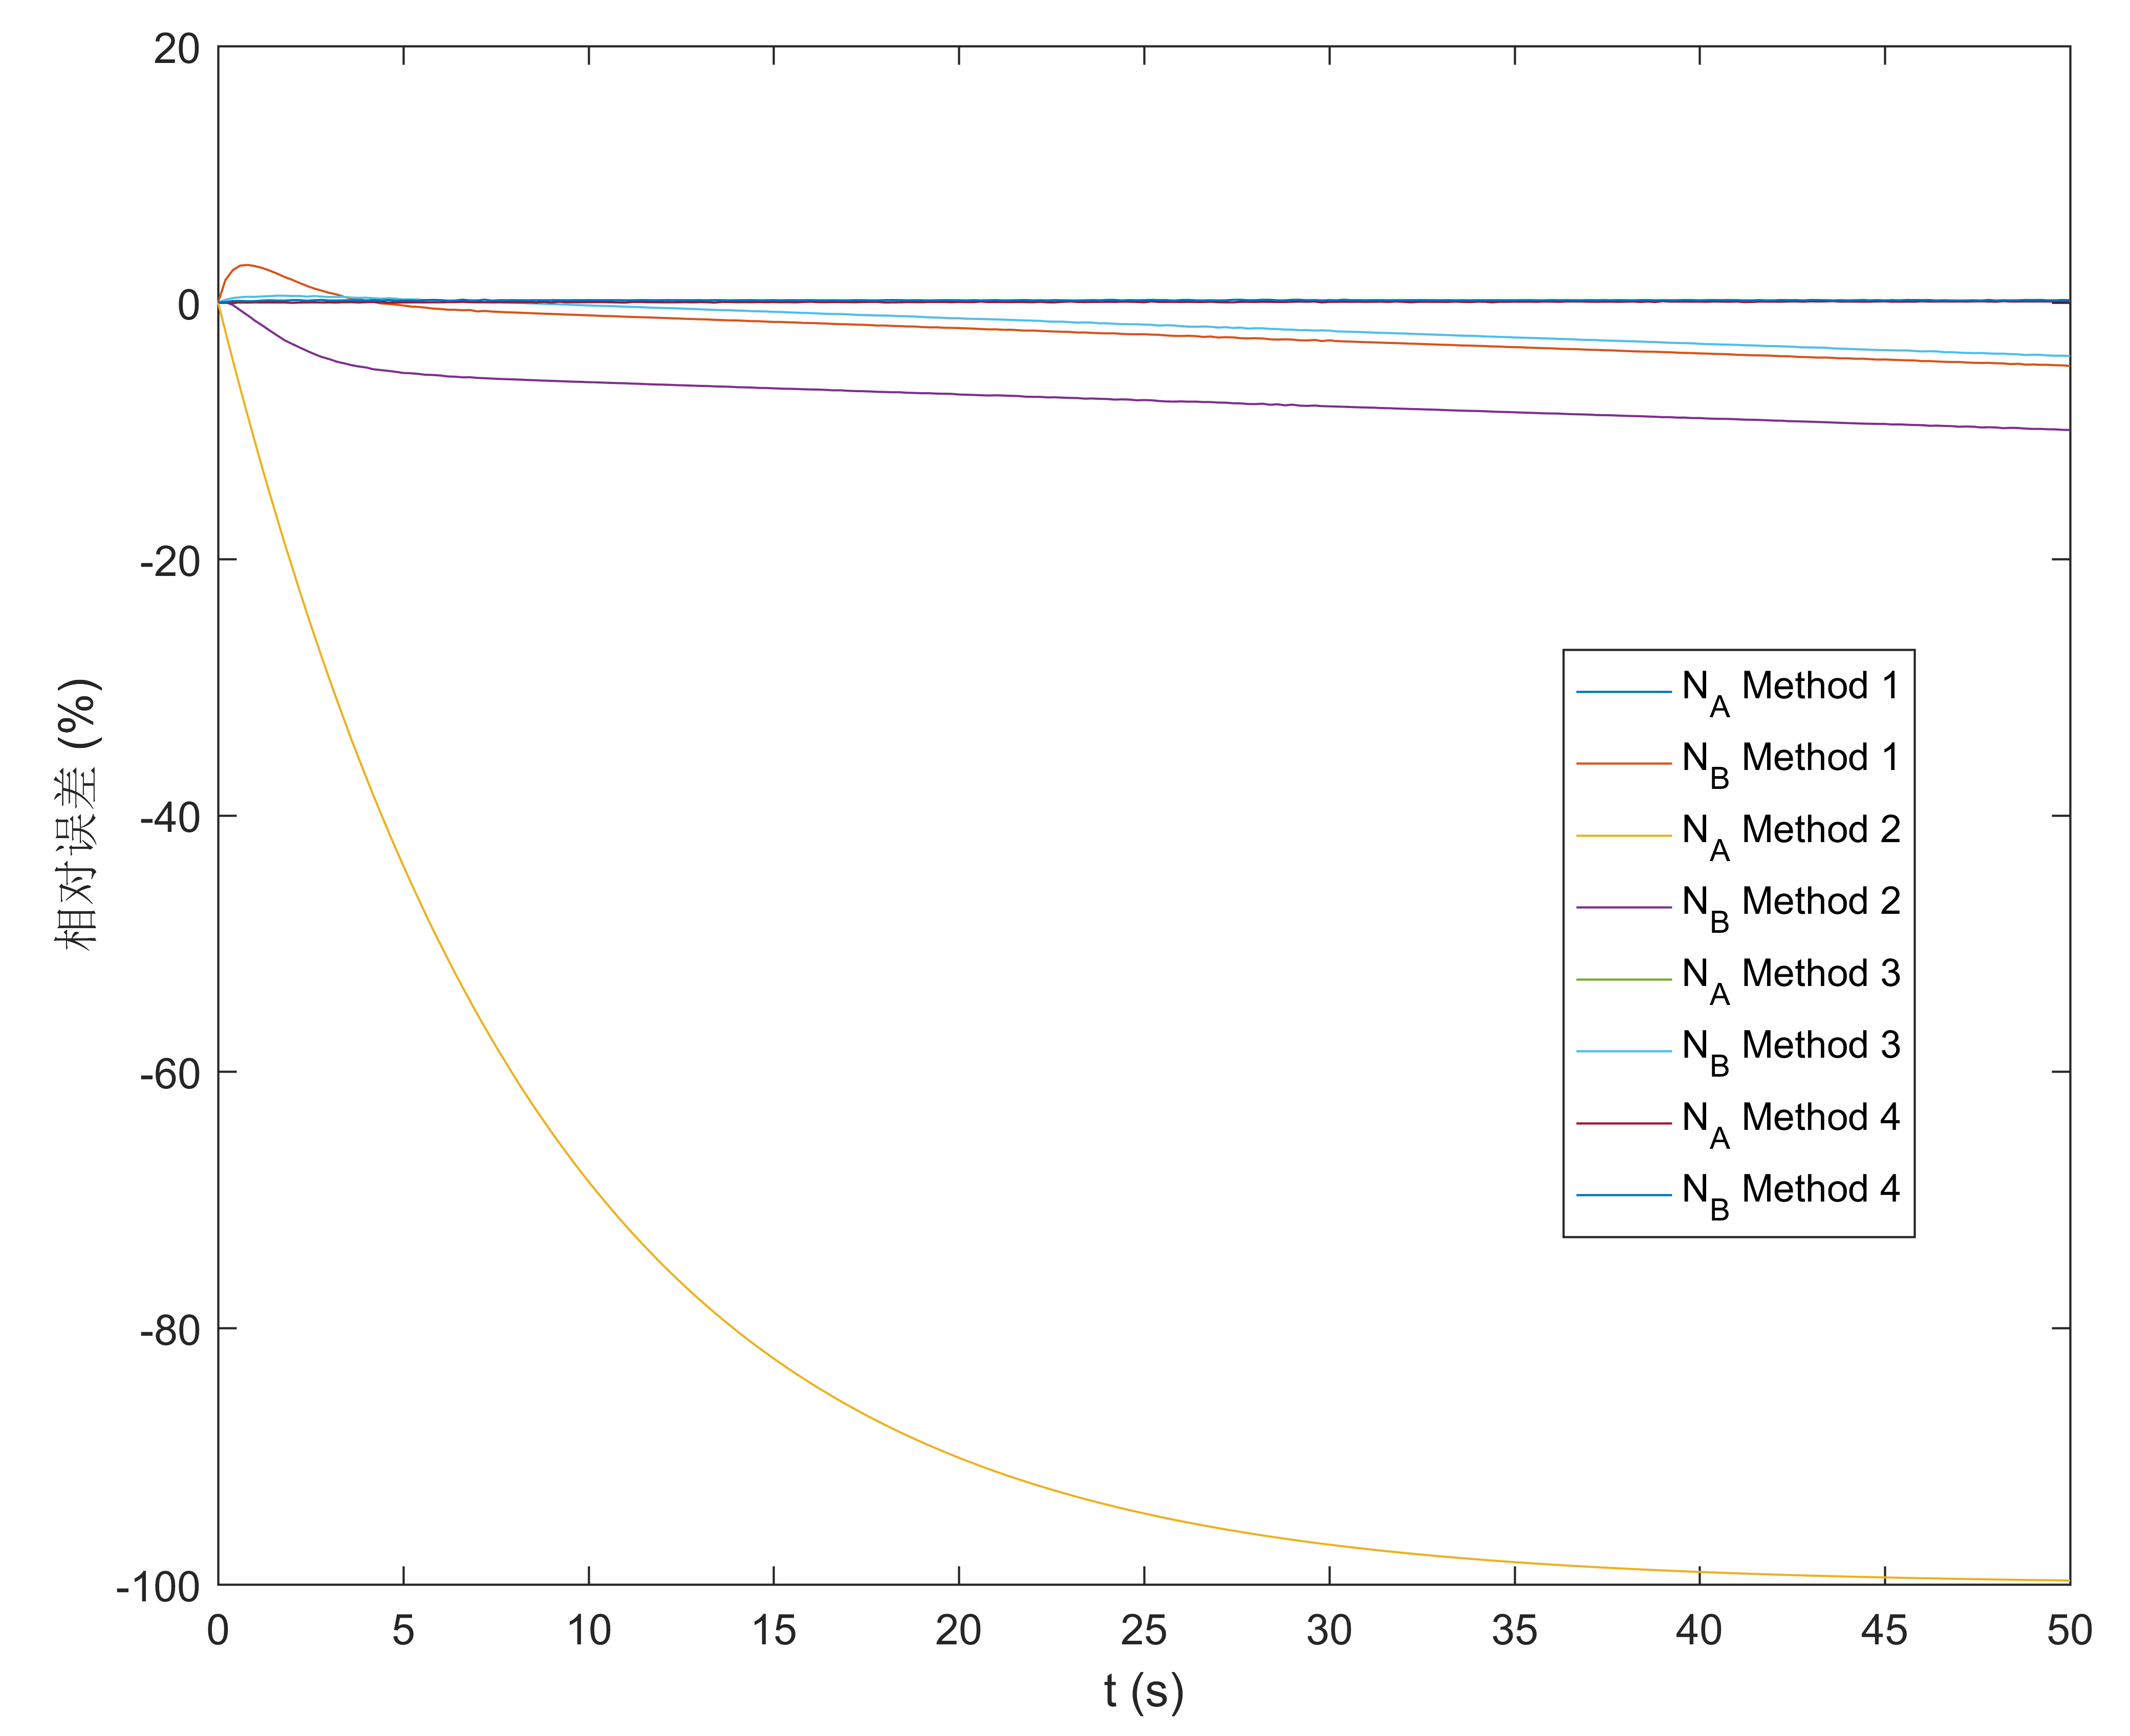
\includegraphics[width=0.6\textwidth]{Q_3_2.png}
	\caption{不同方法在$\tau_{A}=\SI{1}{\second}, \tau_{B}=\SI{10}{\second}, \Delta t=\SI{0.2}{\second}$的情况下的相对误差}
	\label{fig:Q-3-2}
\end{figure}
\begin{figure}[h]
	\centering
	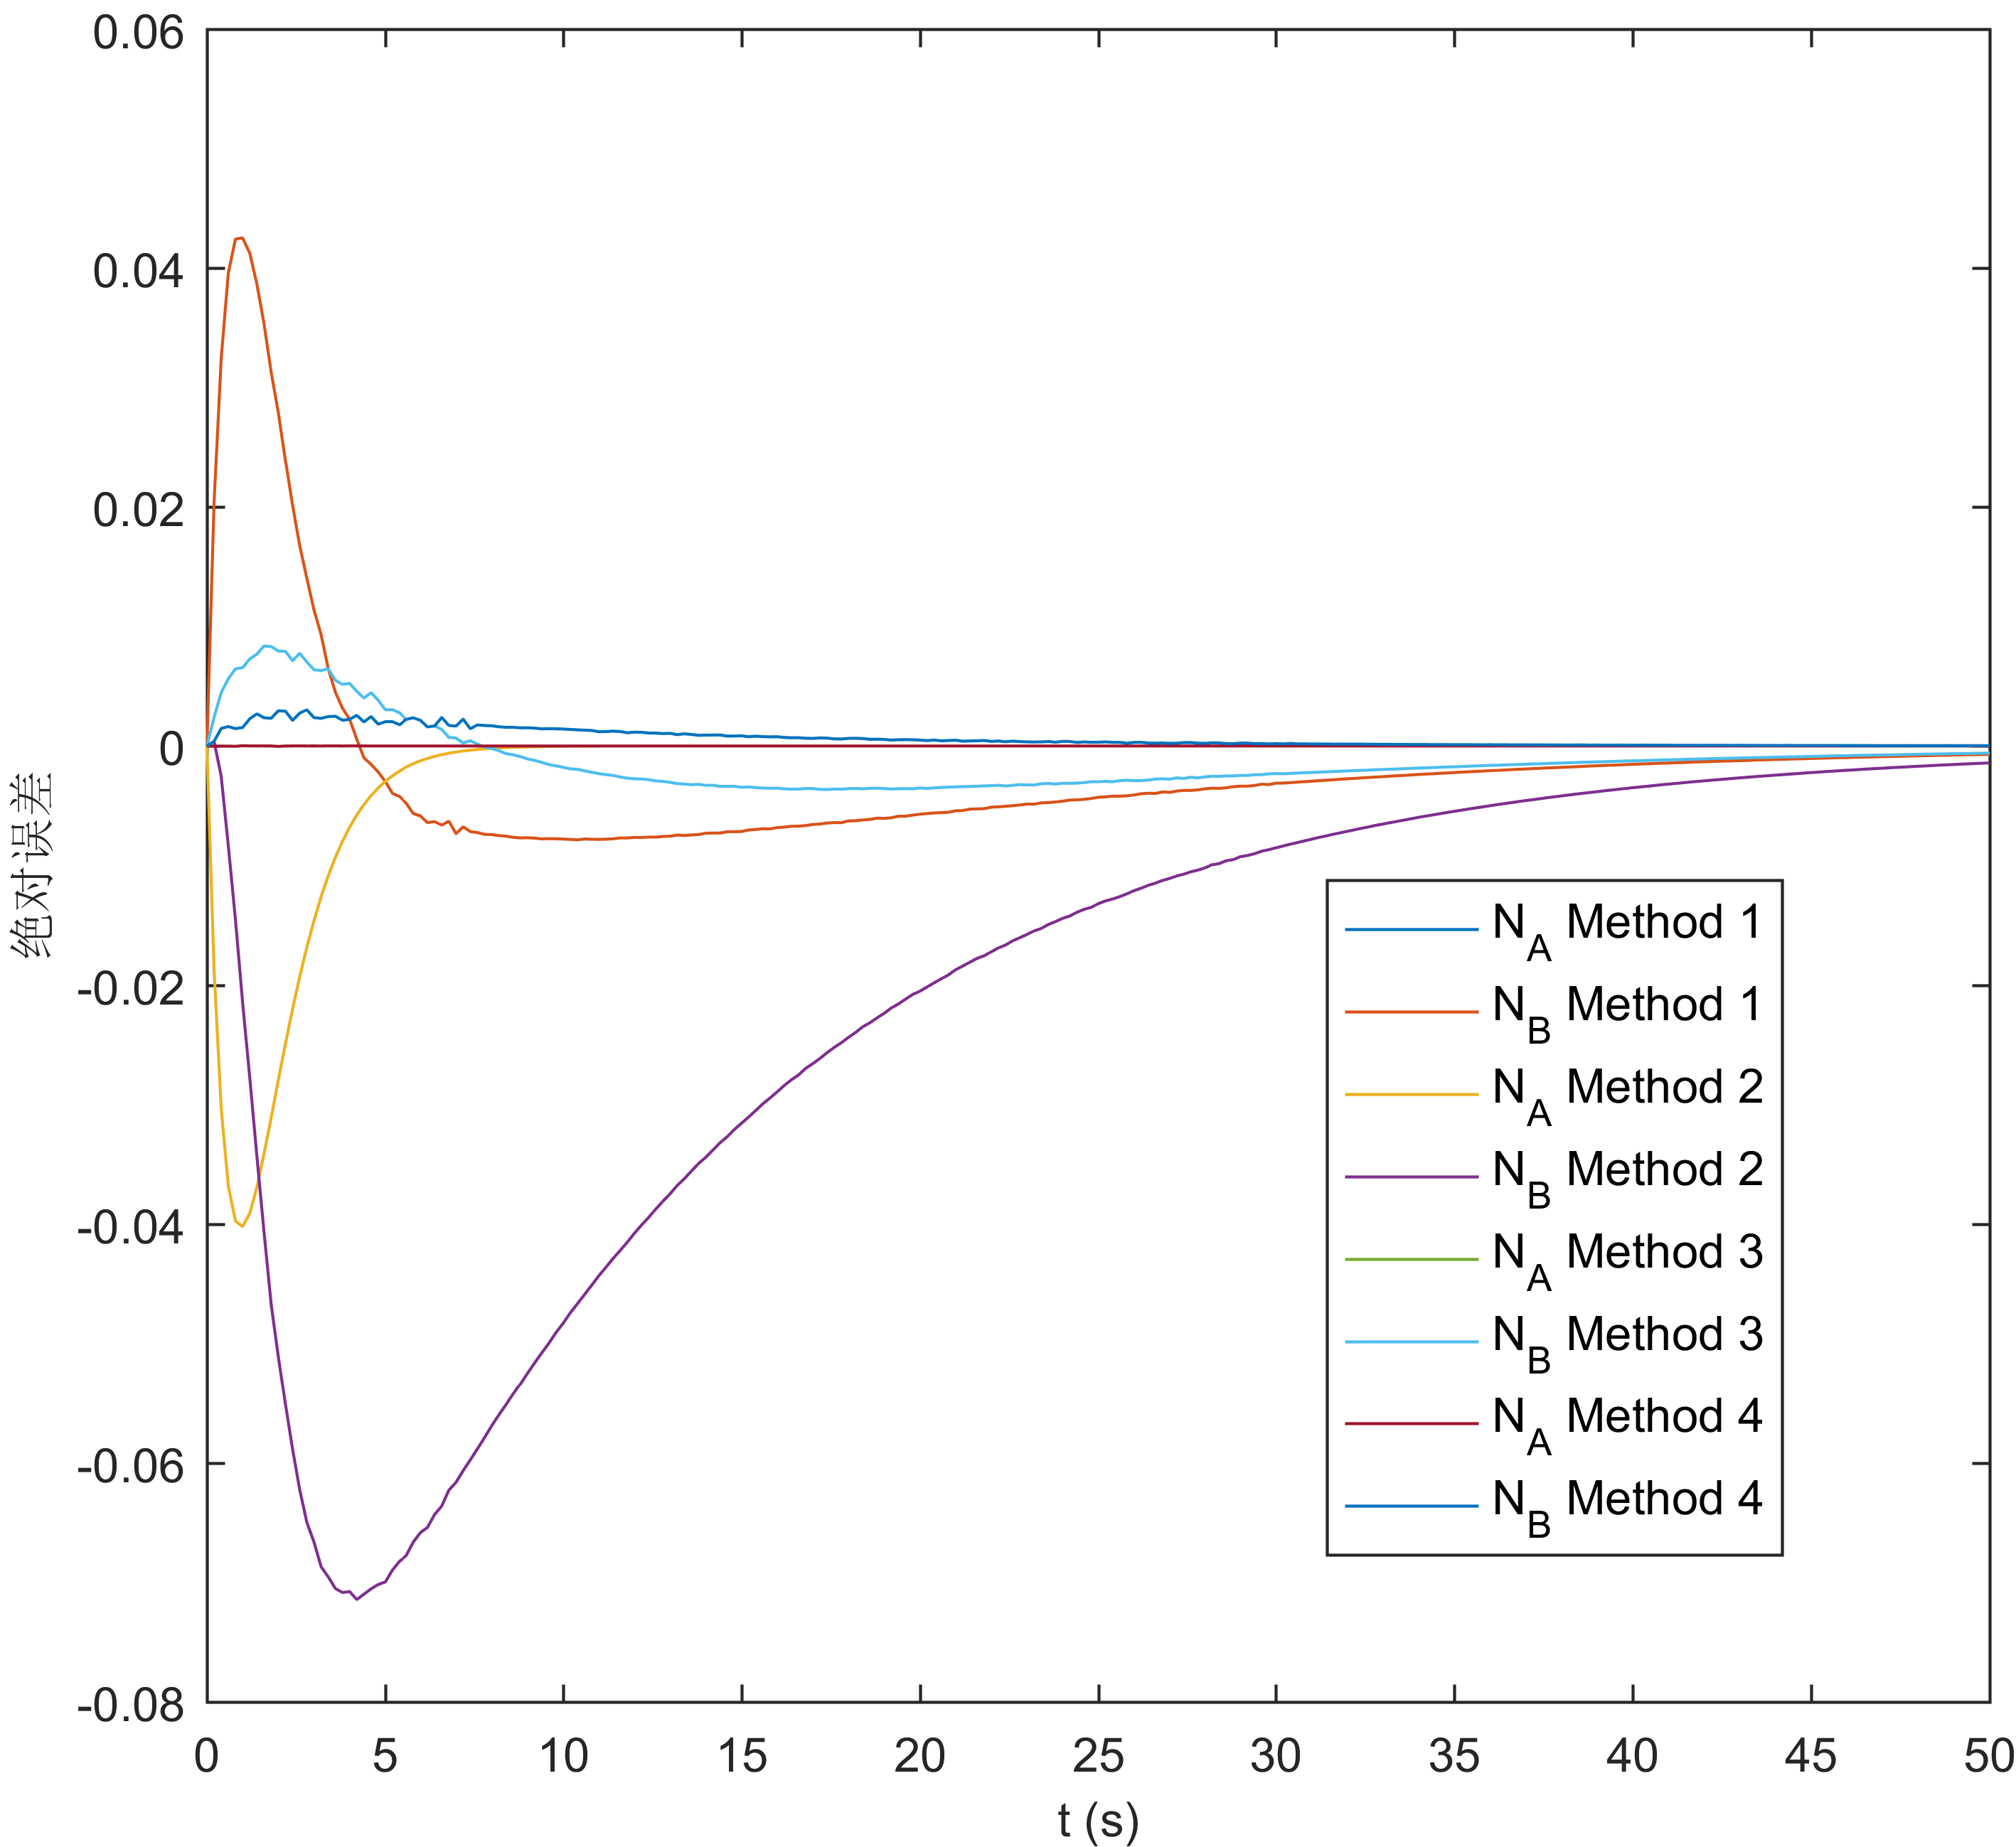
\includegraphics[width=0.6\textwidth]{Q_3_3.png}
	\caption{不同方法在$\tau_{A}=\SI{1}{\second}, \tau_{B}=\SI{10}{\second}, \Delta t=\SI{0.2}{\second}$的情况下的绝对误差}
	\label{fig:Q-3-3}
\end{figure}

\subsection{不同的$\tau_{B}$下的行为}
\begin{figure}[h]
	\centering
	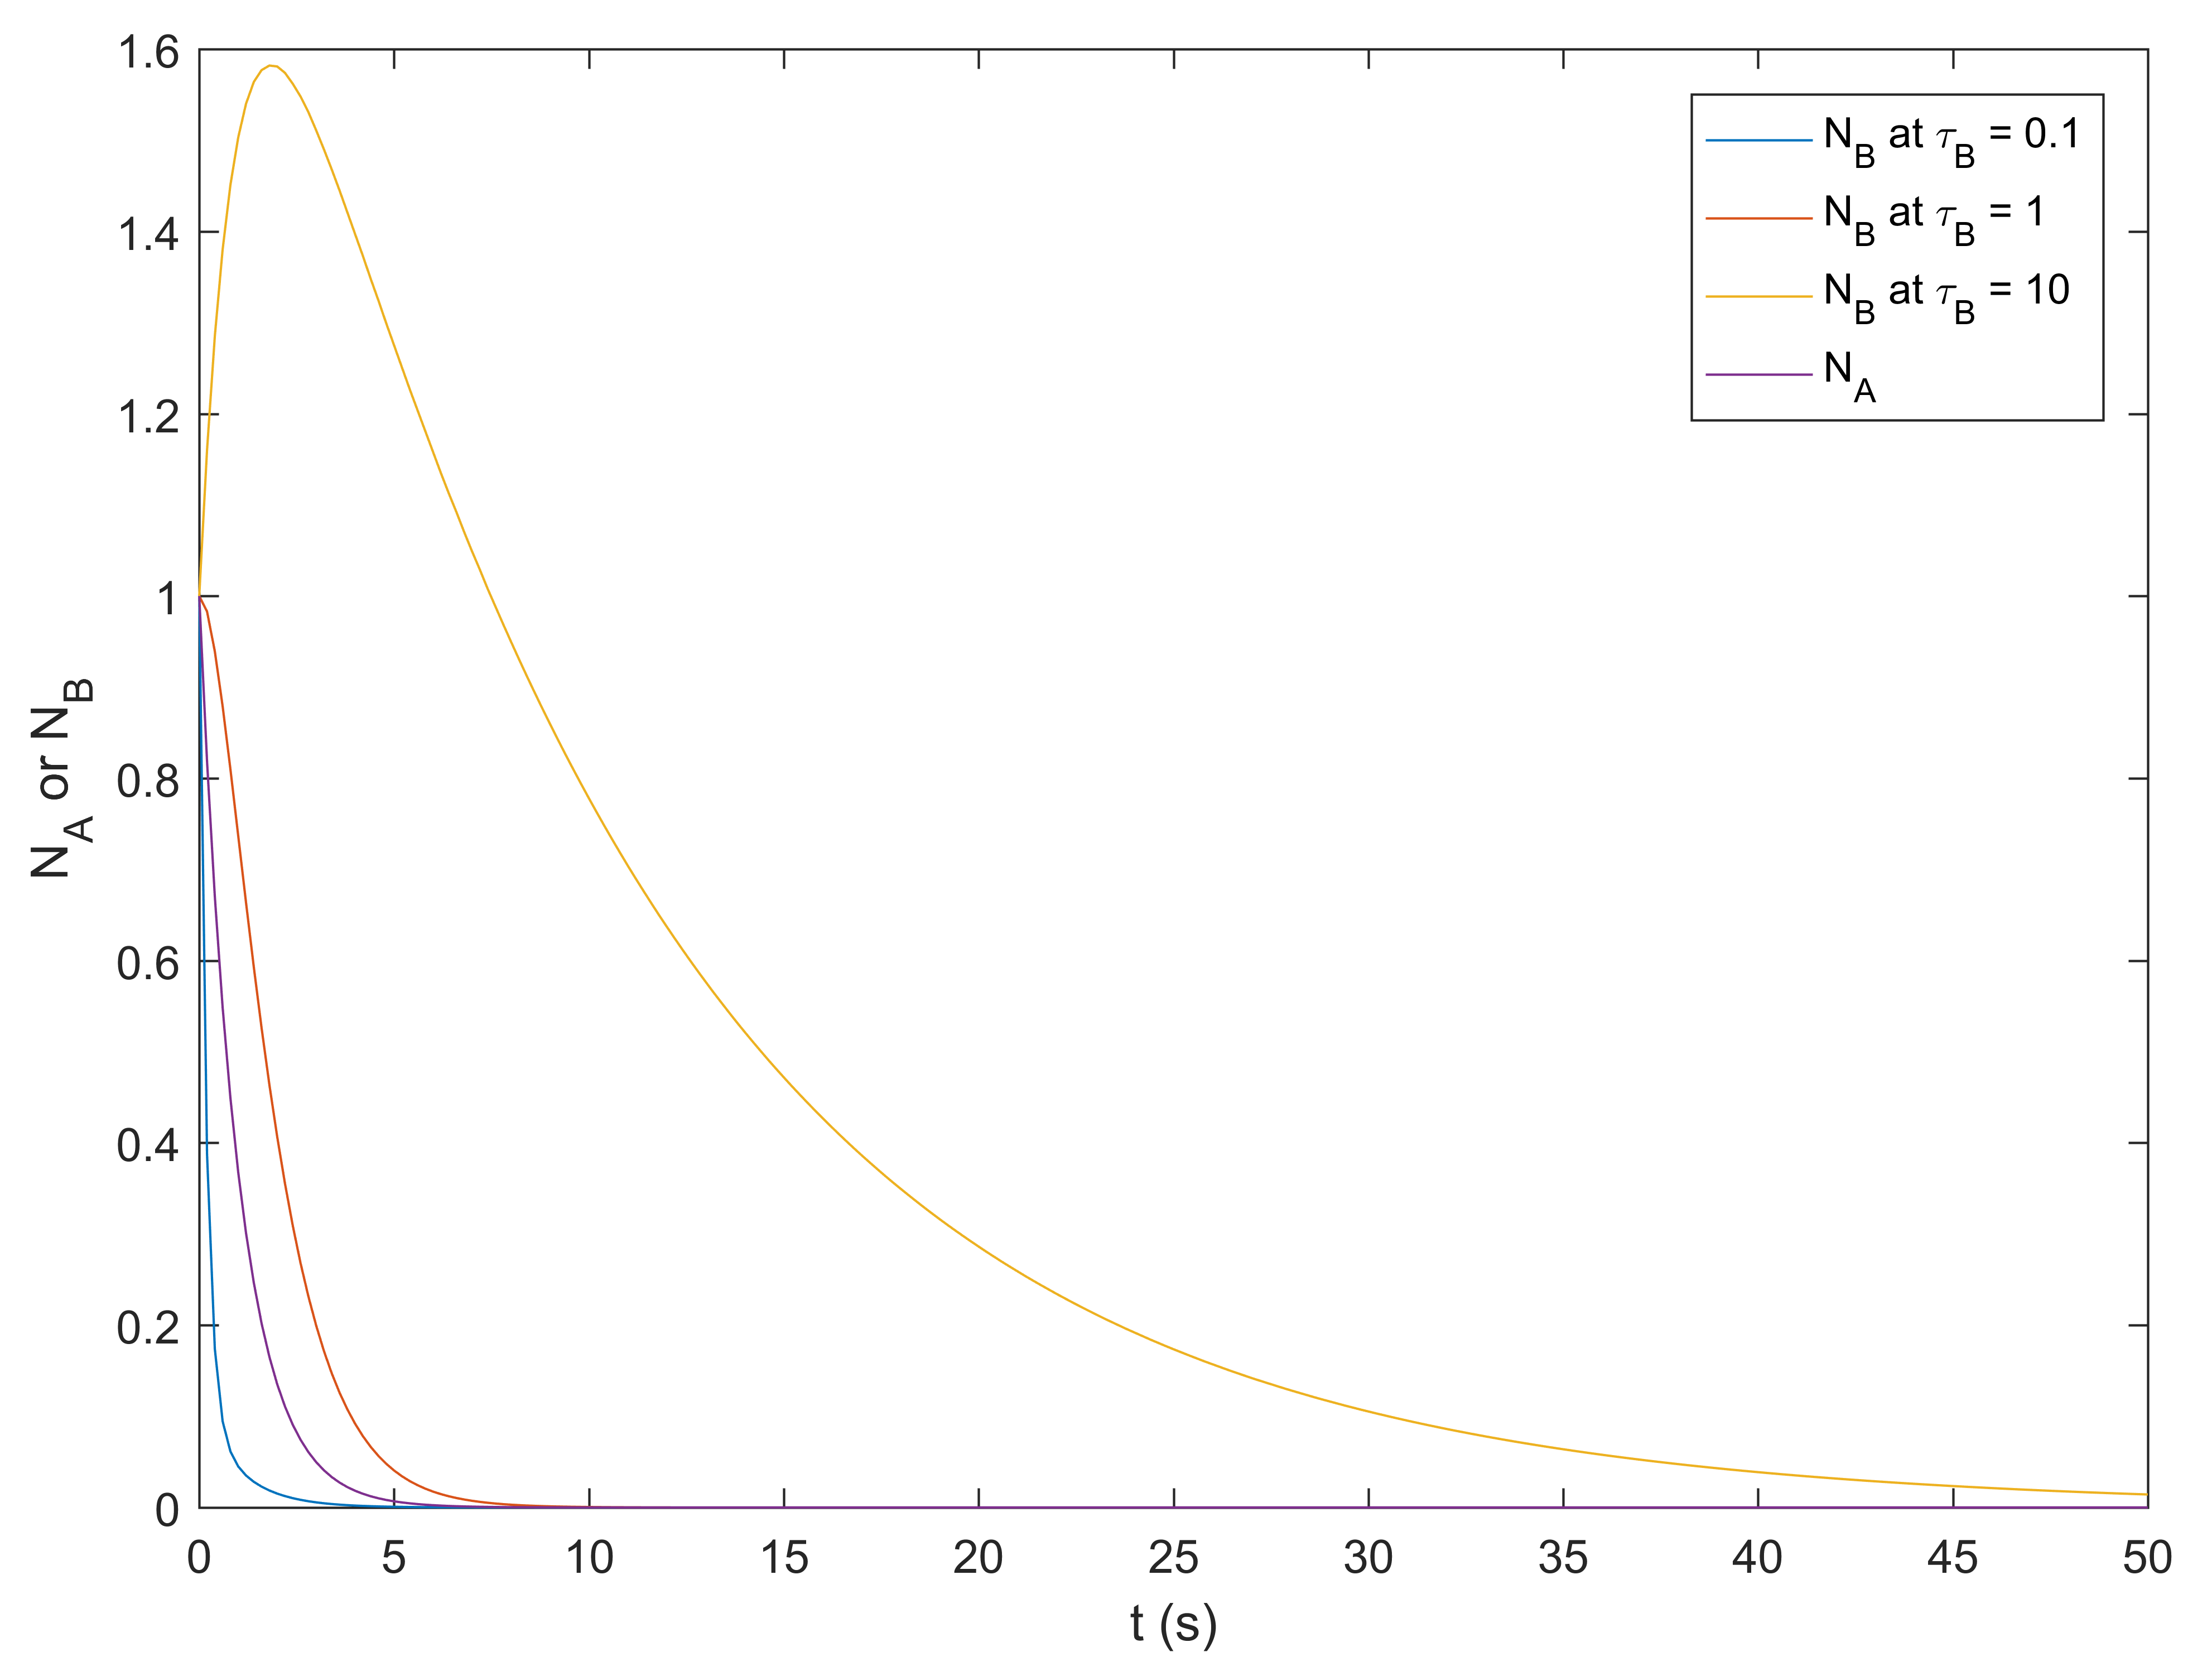
\includegraphics[width=0.7\textwidth]{Q_3_4.png}
	\caption{不同$\tau_{B}$下的结果}
	\label{fig:Q-3-4}
\end{figure}
如图\ref{fig:Q-3-4}所示, $N_A$的行为与$\tau_A$和$\tau_{B}$的大小关系无关,而当$\tau_{B}>\tau_{A}$时,$N_B$短期行为将会出现增加, $\tau_{B}\leqslant\tau_{A}$时,$N_B$将一直减小.$N_B$的长期行为成指数衰减.
\subsection{步长对误差的影响}
表\ref{table:2}给出了$t=\SI{50}{\second}$内不同步长$\Delta t$下的最大相对误差(绝对值). 由于算法本身的误差已经很小,步长变化造成的影响很小,但依然可以看出,步长越小,误差越小.
\begin{table}[h]
	\caption{$t=\SI{50}{\second}$内不同步长$\Delta t$下的最大相对误差(绝对值)}
	\centering
	\vspace{1ex}
	\begin{spacing}{1.5}
	\begin{tabularx}{\textwidth}{CCCC}
		\hline\hline
		$\Delta t$ & $\SI{0.2}{\second}$ & $\SI{0.1}{\second}$ & $\SI{0.05}{\second}$ \\
		\hline
		$N_A$ & 0.103\% & 0.048\% & 0.048\% \\
		$N_B$ & 0.219\% & 0.089\% & 0.057\% \\
		\hline\hline 
	\end{tabularx}
	\end{spacing}
	\label{table:2}
\end{table}
\section{机翼轮廓——插值问题}
\subsection{问题描述}
给定机翼轮廓曲线上的一系列点,利用自然边界条件和三次样条插值方法,绘制出机翼的轮廓.
\subsection{算法}

\subsection{结果}
\subsection{源代码}
\section{双精度浮点数和其IEEE754编码的互相转化}
\subsection{问题描述}
\subsection{算法}
\subsection{结果}
\subsection{源代码}
\clearpage
\appendix
\section{附录}
\subsection{源代码}
\subsubsection{第一题}
\label{subsec:Q_1}
\begin{spacing}{1.0}
	\lstinputlisting[language=C++]{"src/cpp/Problem_1/main.cpp"}
\end{spacing}

\subsubsection{第三题}
\label{subsec:Q_3}
\begin{spacing}{1.0}
	\lstinputlisting[language=C++]{"src/cpp/Problem_3/main.cpp"}
\end{spacing}
\end{document}